\section{Continuity of Functions}
\subsection{Limits of Functions}

Take \(\functiondomain{f}{X}{\CC}\) for some \(X \subseteq \CC\). We want to define what we mean by \(f\pqty{z} \to y\) as \(z \to a\), \emph{even if \(a \notin X\)}.

\begin{figure}[ht!]
    \centering
    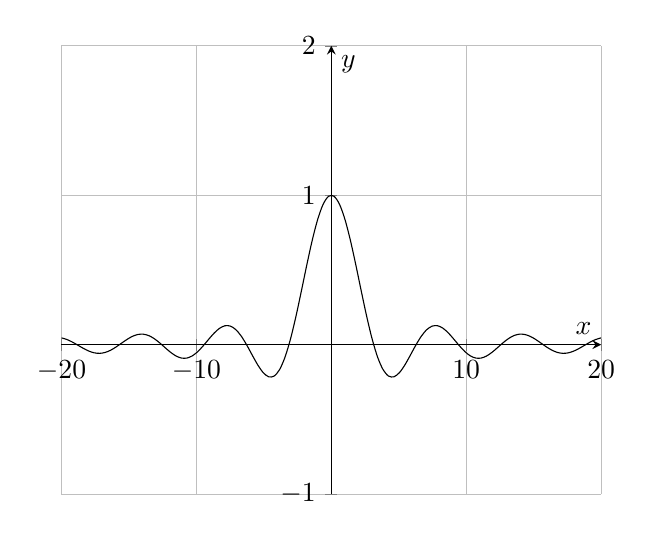
\begin{tikzpicture}[scale=1]
        \begin{axis}[grid=both,
                     xmin=-20, xmax=20, xlabel=\(x\),
                     ymin=-1, ymax=2, ylabel=\(y\),
                    axis lines=center, >=stealth]
        \addplot[domain=-20:20, samples=100] plot[smooth] {sin(deg(x))/x};
        \end{axis}
    \end{tikzpicture}
    \caption{Graph of \(\frac{\sin x}{x}\)}
    \label{fig:graph-sin-x-x}
\end{figure}

\begin{example}[The Function \(\frac{\sin x}{x}\)]
    The function \(f\pqty{x} = \frac{\sin x}{x}\) is not defined at \(x = 0\). But from \autoref{fig:graph-sin-x-x}, we are very tempted to say that this function has a limit of \(1\) as the function tends to \(0\), and if so, we may extend the domain for a new function, to include \(x = 0\) to take a value of \(1\), e.g.,
    \[
        f\pqty{x} = \begin{cases}
            \frac{\sin x}{x}, & x \neq 0, \\
            \lim_{x \to 0} \frac{\sin x}{x}, & x = 0.
        \end{cases}
    \]
\end{example}

The reason why we can hope to make sense of \(\lim_{x \to 0} \frac{\sin x}{x}\) is that there are points that are in the domain that are very close \(0\), and we could jump from points ever closer to \(0\) to get a value for that `limit'.

In other words, \(0\) is an \emph{accumulation point} for \(\RR \setminus \Bqty{0}\): for any threshold \(\delta > 0\), we can always find \(x \in \RR \setminus \Bqty{0}\), such that \(\abs{x - 0} < \delta\).

\begin{definition}[Accumulation and Isolated Point]
    \label{def:fn-accumulation-isolated-point}%
    Let \(X \subseteq \CC\) and \(a \in \CC\). We say \(a\) is an \emph{accumulation point} for \(X\), if that
    \[
        \forall \delta > 0, \exists z \in X \setminus \Bqty{a}: \abs{z - a} < \delta.
    \]

    If \(a \in X\) and it is not an accumulation point, then we say \(a\) is \emph{isolated}.
\end{definition}

\begin{example}[Accumulation and Isolated Point]
    \label{ex:fn-accumulation-isolated-point}%
    \begin{itemize}
        \item The set \(X = \Bqty{0} \cup \ccintv{1}{2}\) has \(0\) as an isolated point. On the other hand, all points in \(\ccintv{1}{2}\) are accumulation points for \(X\).
        \item The points on the unit circle \(S = \set{z \in \CC}{\abs{z} = 1}\) are accumulation points for \(D = \set{z \in \CC}{\abs{z} < 1}\). Also, all the points in \(D\) are also accumulation points for \(D\). \autoref{fig:accumulation-point-c} demonstrates this example.
        \item If we look at \(\set{z \in \CC}{\abs{z} \leq 1}\), then all the points in this set are accumulation points. 
    \end{itemize}
\end{example}

\begin{figure}[ht!]
    \centering
    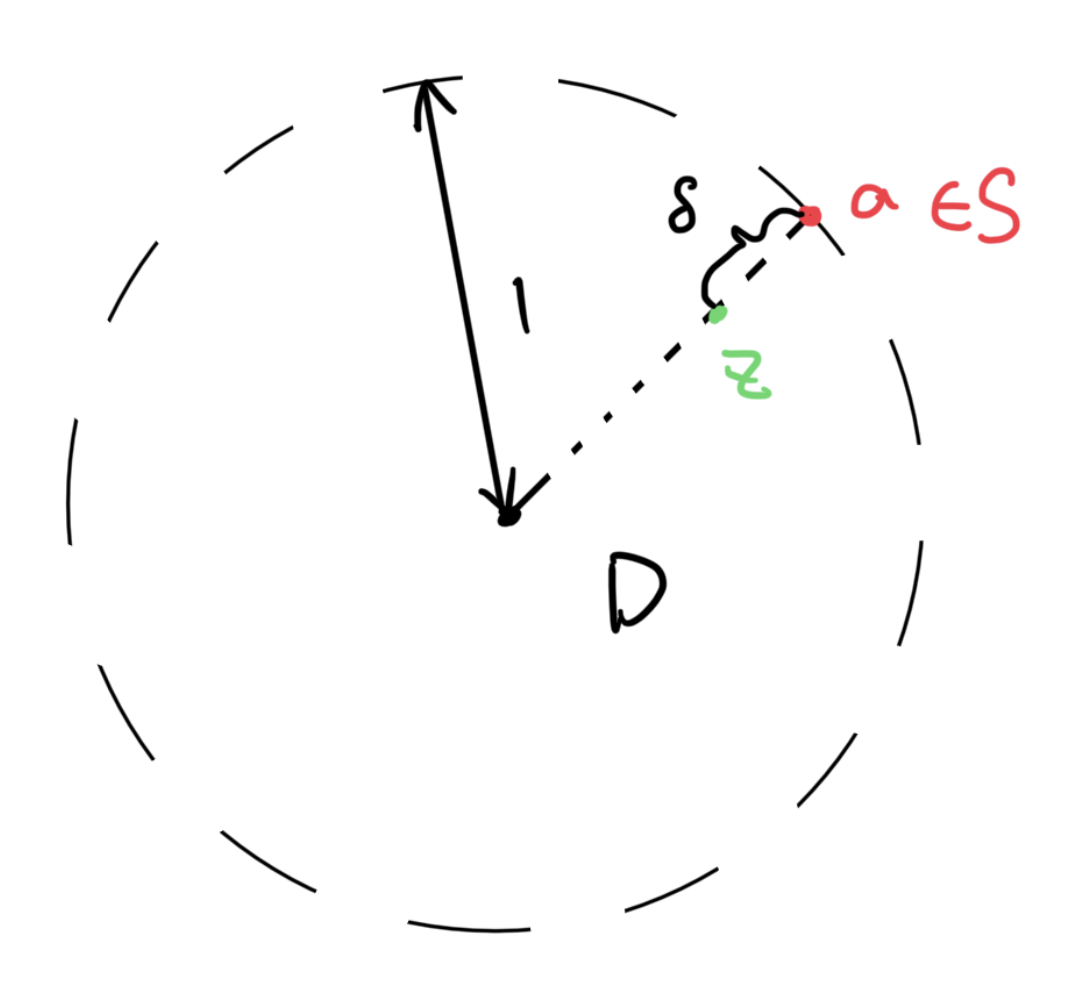
\includegraphics[scale=0.3]{fig/accumulation-points.png}
    \caption{Accumulation Points on Complex Unit Circle}
    \label{fig:accumulation-point-c}
\end{figure}

\begin{lemma}[Accumulation Points are Limit Points]
    Let \(X \subseteq \CC\) and \(a \in \CC\). Then \(a\) is an accumulation point for \(X\) if and only if there exists \(\pqty{x_n}\) in \(X \setminus \Bqty{a}\), such that \(\lim_{n \to \infty} x_n = a\).
\end{lemma}

\begin{proof}
    If there is some \(\pqty{x_n} \subseteq X \setminus \Bqty{a}\) with \(x_n \to a\), then by definition,
    \[
        \forall \epsilon > 0, \exists N = N\pqty{\epsilon} \in \NN, \forall n \geq N: \abs{x_n - a} < \delta.
    \]

    Now, let \(\delta > 0\) be arbitrary, then take \(N = N\pqty{\delta}\), therefore we have \(x_N \in X \setminus \Bqty{a}\) with \(\abs{x_N - a} < \delta\), showing that \(a\) is indeed an accumulation point.

    Conversely, given \(a\) is an accumulation point of \(X\), this means
    \[
        \forall \delta > 0, \exists z = z\pqty{\delta} \in X \setminus \Bqty{a}: \abs{z - a} < \delta.
    \]

    Now, let \(x_n = z\pqty{\frac{1}{n}}\) for \(n \in \NN\), then \(x_n\) is indeed a sequence of \(X \setminus \Bqty{a}\). Therefore,
    \[
        0 < \abs{x_n - a} = \abs{z\pqty{\frac{1}{n}} - a} \leq \frac{1}{n}
    \]
    and by the sandwich theorem, \(\abs{x_n - a} \to 0\), so \(x_n \to a\), as desired.
\end{proof}

Now we return to the definition of a limit. From the point we just saw, we want \(a\) to be an accumulation point of \(X\), since otherwise the behaviour of \(f\) as \(z\) `approaches' \(a\) itself does not make sense -- we need a path for \(z\) to approach the point, via its domain! 

We make sense of \(f\pqty{z}\) as \(z \to a\) by looking at points near \(a\). The idea is, no matter how small the threshold \(\epsilon > 0\), we may let the function be arbitrarily close to \(y\), as long as \(z\) is sufficiently close to \(a\). Formally, we want to define this as follows.

\begin{definition}[Limit of a Function]
    \label{def:fn-limit}%
    Let \(\functiondomain{f}{X \subseteq \CC}{\CC}\). We take some \(a \in \CC\) which is an accumulation point of \(X\).


    We say \(f\) \emph{tends to} \(y \in \CC\) as \(z\) tends to \(a\), if
    \[
        \forall \epsilon > 0, \exists \delta = \delta \pqty{\epsilon} > 0, \forall 0 < \abs{z - a} < \delta, z \in X: \abs{f\pqty{z} - y} < \epsilon,
    \]
    and we denote this as \(f\pqty{z} \to y\) as \(z \to a\), or \(\lim_{z \to a} f\pqty{z} \to y\).

    Similarly, we say \(f\) diverges to \(\infty\) as \(z \to a\), if
    \[
        \forall L > 0, \exists \delta = \delta\pqty{L} > 0, \forall 0 < \abs{z - a} < \delta, z \in X: \abs{f\pqty{z}} > L.
    \]
\end{definition}

\begin{remark}
    \begin{itemize}
        \item We shall not worry about the limit at an isolated point, since there is not a good behaviour of `approaching' \(a\) in any sense. (Indeed, most of the following results on limits only concerns accumulation points.) Therefore, some choose to not define the limit at an isolated point, while others might choose to define \(\lim_{z \to a} f\pqty{z} = f\pqty{a}\). The latter might be chosen since it would make the limit condition for \autoref{def:fn-continuity} (Continuity) work for isolated points as well.
        
        In particular, our definition does not work well for isolated points, since for sufficiently small \(\delta\), there is no \(z \in X\) such that \(0 < \abs{z - a} < \delta\), and our condition is trivially true for \emph{any} \(y\) which is not what we want.

        \item Note that \(f\) may diverge to infinity at \(a \in \CC\), even with \(a \in X\). Consider the example
        \[
            f\pqty{x} = \begin{cases}
                \frac{1}{x^2}, & x \neq 0, \\
                0, & x = 0,
            \end{cases}  
        \]
        and at \(x = 0\), \(f\pqty{0} = 0\) but
        \[
            \lim_{x \to 0} f\pqty{x} \to \infty.
        \]
    \end{itemize}
\end{remark}

\begin{example}[\(\frac{\sin x}{x}\) as \(x \to 0\)]
    \label{ex:sin-x-x-limit}%
    We claim that \(\frac{\sin x}{x} \to 1\) as \(x \to 0\). Using trigonometry, we have that
    \[
        \cos x < \frac{\sin x}{x} < 1
    \]
    for all \(x \in \oointv{0}{\frac{\pi}{2}}\). Hence,
    \[
        \abs{\frac{\sin x}{x} - 1} < 1 - \cos x = 2 \sin^2 \pqty{\frac{x}{2}} < \frac{x^2}{2}.
    \]

    Hence, for all \(\epsilon > 0\), we choose \(\delta\pqty{\epsilon} = \sqrt{2\epsilon}\), and hence
    \[
        \abs{x - 0} < \delta \implies \abs{\frac{\sin x}{x} - 1} < \frac{\pqty{\sqrt{2 \epsilon}}^2}{2} = \epsilon
    \]
    for \(x > 0\), and since this function is even, the same behaviour holds for \(x < 0\), which finishes our proof.
\end{example}

\begin{lemma}[Sequential Limits / Heine's Theorem]
    \label{lem:fn-sequential-limits}%
    Let \(\functiondomain{f}{X \subseteq \CC}{\CC}\), and let \(a \in \CC\) be an accumulation point of \(X\). Then
    \[
        \lim_{z \to a} f\pqty{z} = y
    \]
    if and only if
    \[
        \lim_{n \to \infty} f\pqty{z_n} = y
    \]
    for any \(\pqty{z_n}\) on \(X \setminus \Bqty{a}\), with \(z_n \to a\).

    Similarly, \(f\pqty{z}\) diverges to infinity, if and only if \(\pqty{f\pqty{z_n}}\) diverges to infinity for every \(\pqty{z_n}\) on \(X \setminus \Bqty{a}\), with \(z_n \to a\).
\end{lemma}

\begin{proof}
    We prove for convergence, and the case for divergence is similar.
    
    Suppose that \(\lim_{z \to a} f\pqty{z} = y\). Let \(\epsilon > 0\) be arbitrary, and let \(\delta > 0\) be such that
    \[
        \forall z \in X, 0 < \abs{z - a} < \delta: \abs{f\pqty{z} - y} < \epsilon.
    \]

    Now, take any \(\pqty{z_n} \to a\) on \(X \setminus \Bqty{a}\). Since \(\delta > 0\), there is some \(N > 0\) such that
    \[
        \forall n \geq N: 0 < \abs{z_n - a} < \delta.
    \]

    Hence,
    \[
        \forall n \geq N: \abs{f\pqty{z_n} - y} < \epsilon
    \]
    showing that the limit of the sequence converges as desired.

    Conversely, we prove using the contrapositive, so suppose \(\lim_{z \to a} f\pqty{z} \neq y\). Then for some \(\epsilon > 0\), we have for all \(\delta > 0\), we have
    \[
        \exists z \in X, 0 < \abs{z - a} < \delta: \abs{f\pqty{z} - y} \geq \epsilon.
    \]

    Taking \(\delta = 1, \frac{1}{2}, \frac{1}{3}, \ldots\), we construct a sequence of such \(z_n \in X\), and we have for all \(n \in \NN\),
    \[
        z_n \in X \qand 0 < \abs{z_n - a} < \frac{1}{n}
    \]
    which shows \(\pqty{z_n} \to a\) on \(X \setminus a\), and indeed,
    \[
        \abs{f\pqty{z_n} - y} \geq \epsilon,
    \]
    which shows that \(f\pqty{z_n} \notto y\). This finishes the proof.
\end{proof}

\begin{lemma}[Limit of Function is Unique]
    \label{lem:fn-limit-unique}%
    If \(\functiondomain{f}{X \subseteq \CC}{\CC}\) has a limit at \(a \in \CC\), then this limit is unique.
\end{lemma}

\begin{proof}[\proofname\ using Sequences]
    This is a corollary of \autoref{lem:fn-sequential-limits} due to the uniqueness of the limit of a sequence.
\end{proof}

\begin{proof}[\proofname\ using \(\epsilon-\delta\)]
    Suppose that \(f\pqty{z} \to y\) and \(f\pqty{z} \to x\) as \(z \to a\). We have that
    \[
        \abs{x - y} \leq \abs{x - f\pqty{z}} + \abs{f\pqty{z} - y}
    \]
    and using similar techniques in \autoref{lem:seq-limit-unique} (Sequences have Unique Limit), we have \(x = y\).
\end{proof}

\begin{lemma}[Function Limits Preserve Arithmetic]
    \label{lem:fn-limits-preserve-arithmetic}%
    Let \(\functiondomain{f, g}{X \subseteq \CC}{\CC}\), and \(a \in \CC\) be an accumulation point of \(X\). Suppose \(\lim_{z \to a} f\pqty{z} = a\) and \(\lim_{z \to a} g\pqty{z} = b\), then
    \begin{align*}
        \lim_{x \to a} \pqty{f\pqty{z} + g\pqty{z}} &= a + b, \\
        \lim_{x \to a} \pqty{f\pqty{z} \cdot g\pqty{z}} & = ab.
    \end{align*}

    Furthermore, if \(b \neq 0\), we have
    \[
        \lim_{z \to a} \frac{f\pqty{z}}{g\pqty{z}} = \frac{a}{b}.
    \]
\end{lemma}

\begin{proof}
    The techniques in proving this is similar to what we did in \autoref{lem:seq-limits-arithmetic} (Limit of Sequence Preserve Arithmetic), so we will not repeat the proof here.
\end{proof}

\subsection{Continuity of Functions}

\begin{definition}[Continuity]
    \label{def:fn-continuity}%
    Let \(\functiondomain{f}{X \subseteq \CC}{\CC}\).

    We say \(f\) is \emph{continuous at some point \(a \in X\)}, if
    \[
        \forall \epsilon > 0, \exists \delta = \delta\pqty{\epsilon}, \forall \abs{z - a} < \delta, z \in X: \abs{f\pqty{z} - f\pqty{a}} < \epsilon.
    \]

    
    
    We say \(f\) is \emph{continuous} if it is continuous at every point in \(X\).    
\end{definition}

\begin{remark}
    If \(a \in X\) is an isolated point, \(f\) is then trivially continuous at \(a\), because for sufficiently small \(\delta\), \(\abs{z - a} < \delta\) implies \(z = a\), so \(f\pqty{z} = f\pqty{a}\).

    On the other hand, if \(a \in X\) is an accumulation point, this is equivalent to saying
    \[
        \lim_{z \to a} f\pqty{z} = f\pqty{a}.
    \] 
\end{remark}

\begin{example}[Examples on Continuity]
    \label{ex:fn-continuity}
    \begin{itemize}
        \item \(f\pqty{z} = z\) is the identity function. This is continuous everywhere on the domain, say \(\CC\). For all \(\epsilon > 0\), we choose \(\delta = \epsilon\), so for all \(\abs{z - a} < \delta\), we have \(\abs{f\pqty{z} - f\pqty{a}} = \abs{z - a} < \delta = \epsilon\).

        \item If \(\functiondomain{f}{\RR}{\RR}\) satisfies \[
            f\pqty{x} = \begin{cases}
                \sin \pqty{\frac{1}{x}}, & x \neq 0, \\
                0, & x = 0,
            \end{cases}
        \]
        then \(f\) is not continuous at \(0\).
    \end{itemize}
\end{example}

To show the second example, it would be helpful to have another definition of continuity.

\begin{definition}[Sequential Continuous]
    \label{def:fn-sequential-continuous}%
    Let \(\functiondomain{f}{X \subseteq \CC}{\CC}\). We say \(f\) is \emph{sequential continuous} at \(a \in X\), if \(f\pqty{z_n} \to f\pqty{a}\) (as a sequence) for any \(\pqty{z_n}\) on \(X\) such that \(z_n \to a\).
\end{definition}

\begin{proposition}[Sequential Continuity is Continuity]
    \label{prop:fn-seq-cont-iff-cont}%
    Let \(\functiondomain{f}{X \subseteq \CC}{\CC}\) and \(a \in X\). \(f\) is continuous at \(a\) if and only if \(f\) is sequentially continuous at \(a\).
\end{proposition}
We now prove the proposition.

\begin{proof}[\proofname\ of \autoref{prop:fn-seq-cont-iff-cont} (Sequential Continuity), by Definition]
    We first show continuity implies sequential continuity. By continuity, for \(\epsilon > 0\), we have \(\delta = \delta\pqty{\epsilon} > 0\) such that
    \[
        \abs{z - a} < \delta \implies \abs{f\pqty{z} - f\pqty{a}} < \epsilon.
    \]

    Take \(\pqty{z_n}\) on \(X\) with \(z_n \to a\). By the definition of a sequence limit, there is some \(N = N\pqty{\epsilon} > 0\) such that
    \[
        n \geq N \implies \abs{f\pqty{z_n} - f\pqty{a}} < \epsilon,
    \]
    so we are done.

    We show the converse by contrapositive. Suppose \(f\) instead is not continuous at \(a\). Then by definition, for some \(\epsilon > 0\), we have
    \[
        \forall \delta > 0, \exists z = z\pqty{\delta} \in X, \abs{z - a} < \delta: \abs{f\pqty{z} - f\pqty{a}} \geq \epsilon.
    \]

    Take \(\delta = 1, \frac{1}{2}, \frac{1}{3}, \ldots, \frac{1}{n}, \ldots\) to find \(\pqty{z_n}\), by taking
    \[
        z_n = z \pqty{\frac{1}{n}},
    \]
    and we have
    \[
        \abs{f\pqty{z_n} - f\pqty{a}} \geq \epsilon.
    \]

    \(f\) is not sequentially continuous, as desired.
\end{proof}

\begin{proof}[\proofname\ of \autoref{prop:fn-seq-cont-iff-cont} (Sequential Continuity), using Sequential Limits]
    The result is trivial on isolated points since the only sequence converging to an isolated point in the set is eventually the constant sequence at the point itself, and a function is trivially continuous at isolated points.

    For accumulation points, this can be deduced from \autoref{lem:fn-sequential-limits} (Sequential Limits) and the definition of continuity using a limit. 
    
    Concretely, if \(f\) is sequential continuous, then taking any sequence \(\pqty{z_n}\) on \(X \setminus \Bqty{a}\) with \(z_n \to a\) will give \(f\pqty{z_n} \to f\pqty{a}\), showing that \(f\pqty{z} \to f\pqty{a}\), which gives continuity at an accumulation point.

    Now assume \(f\) is continuous. For any sequence \(\pqty{z_n}\) on \(X\) with \(z_n \to a\), removing terms where \(z_n = a\) would not affect \(z_n \to a\). After removing these terms, we get a sequence \(\pqty{z'_n}\), and by considering the sequential limit (using continuity), we have \(f\pqty{z'_n} \to f\pqty{a}\). But now, adding those terms where \(z_n = a\) back to the sequence does not affect \(f\pqty{z'_n} \to f\pqty{a}\). This indeed shows sequential continuity.
\end{proof}

Using \autoref{prop:fn-seq-cont-iff-cont} (Sequential Continuity), we may show indeed that the second example of \autoref{ex:fn-continuity} is not continuous at \(0\). Let \(\pqty{x_n}\) on \(\RR\) with \(x_n \to 0\), given by
\[
    x_n = \frac{1}{\pqty{2n + \frac{1}{2}} \pi}
\]
and hence
\[
    f\pqty{x_n} = \sin\pqty{\pqty{2n + \frac{1}{2}} \pi} = 1
\]
and in particular, \(f\pqty{x_n} \to 1 \neq 0\).

\begin{examples}[Continuity, Continued]
    \label{ex:continuity-continued}%
    \begin{itemize}
        \item Let
        \[
            \function{f}{\RR}{\Bqty{0, 1}}
            {x}{\indicator_{\QQ} \pqty{x} = \begin{cases}
                1, & x \in \QQ, \\
                0, & x \in \RR \setminus \QQ.
            \end{cases}}
        \]

        This is discontinuous at every point \(a \in \RR\).

        \begin{itemize}
            \item If \(a \in \QQ\), take some irrational sequence \(\pqty{x_n}\) on \(\RR \setminus \QQ\) with \(x_n \to a\). Then
            \[
                f\pqty{x_n} = 0 \to 0 \neq 1 = f\pqty{a}.
            \]
            \item If \(a \in \RR \setminus \QQ\), taking a rational sequence with the same technique tells us that it cannot be continuous there either.
        \end{itemize}

        \item The function \(f\pqty{x} = \sin x\) for \(x \in \RR\) is continuous. Fix \(a \in \RR\), we have
        \begin{align*}
            \abs{f\pqty{x} - f\pqty{a}} &= \abs{\sin x - \sin a} \\
            &\leq 2 \abs{\cos \pqty{\frac{x + a}{2}} \sin \pqty{\frac{x - a}{2}}} \\
            &\leq 2 \abs{\sin \pqty{\frac{x - a}{2}}} \\
            &\leq \abs{x - a},
        \end{align*}
        for \(\frac{x - a}{2} \in \ccintv{-\frac{\pi}{2}}{\frac{\pi}{2}}\). Therefore, for any \(\epsilon > 0\), we choose \(\delta\pqty{\epsilon} = \min\Bqty{\epsilon, \frac{\pi}{2}}\), and this shows continuity. Alternatively, we may also show this using sequential limits.
    \end{itemize}
\end{examples}

Now we show standard properties of continuity.

\begin{lemma}[Continuity is Preserved in Arithmetic]
    \label{lem:fn-continuity-arithmetic}%
    Let \(\functiondomain{f, g}{X \subseteq \CC}{\CC}\) be continuous at \(a \in X\). Then the sum \(f\pqty{x} + g\pqty{x}\), the product \(f\pqty{x}g\pqty{x}\), and the reciprocal \(\frac{1}{f\pqty{x}}\) (if \(f\pqty{a} \neq 0\)) are continuous at \(a\).
\end{lemma}

\begin{proof}
    If \(a\) is an isolated point, this is trivially true. If \(a\) is an accumulation point, this follows from \autoref{lem:fn-limits-preserve-arithmetic} (Function Limits Preserve Arithmetic) using the definition of continuity using a limit.
\end{proof}

\begin{lemma}[Composition of Continuous Functions is Continuous]
    \label{lem:fn-composition-continuous}%
    Let \(U, V \subseteq \CC\), and \(\functiondomain{f}{U}{V}\), \(\functiondomain{g}{V}{\CC}\). If \(f\) is continuous at \(a \in U\), and \(g\) is continuous at \(f\pqty{a} \in V\), then \(\functiondomain{g \circ f}{U}{\CC}\) is continuous at \(a\).
\end{lemma}

\begin{figure}[ht!]
    \centering
    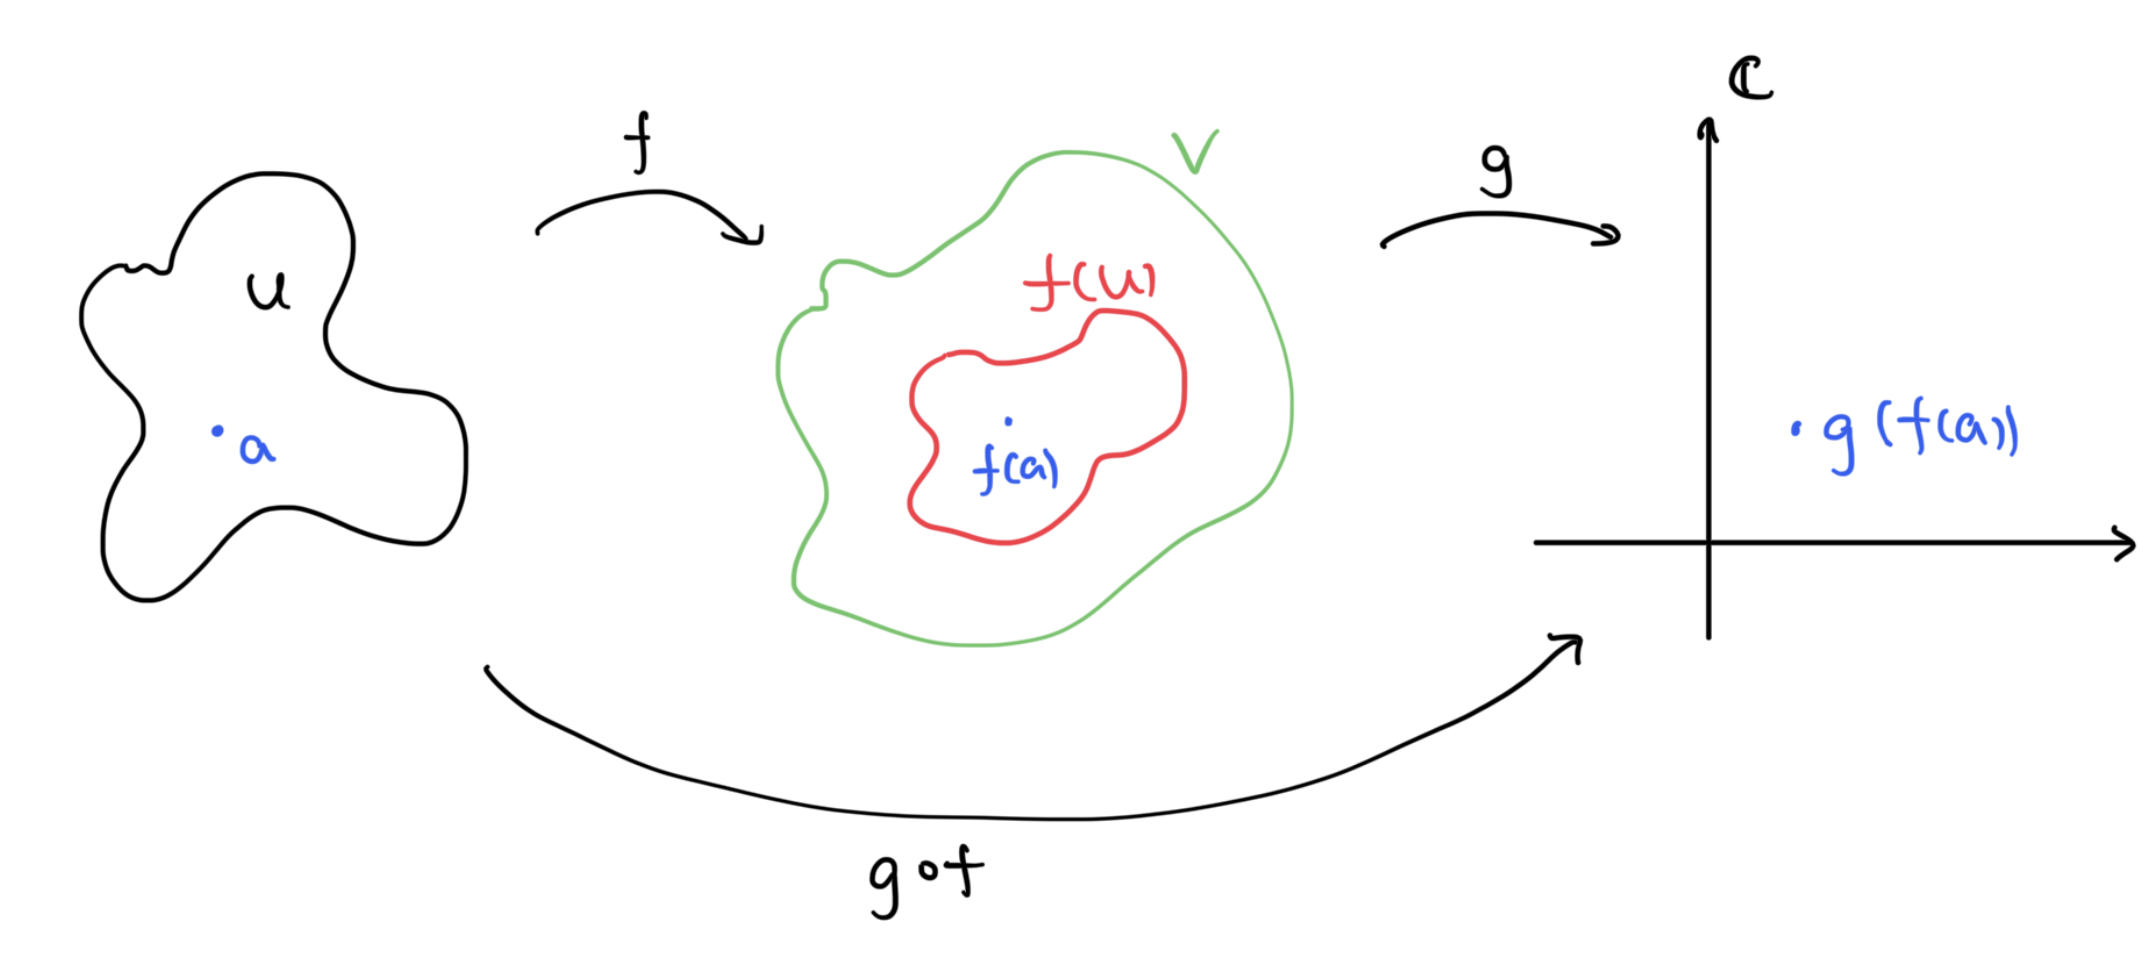
\includegraphics[scale=0.4]{fig/function-composition-continuity.png}
    \caption{Function Composition preserves Continuity}
    \label{fig:fn-composition-continuous}%
\end{figure}

\autoref{fig:fn-composition-continuous} visualises the condition required in \autoref{lem:fn-composition-continuous}.

\begin{proof}
    Since \(g\) is continuous at \(f\pqty{a}\), for \(\epsilon > 0\), we have some \(\sigma = \sigma\pqty{\epsilon} > 0\), such that
    \[
        y \in V, \abs{y - f\pqty{a}} < \sigma \implies \abs{g\pqty{y} - g\pqty{f\pqty{a}}} < \epsilon.
    \]

    On the other hand, since \(f\) is continuous at \(a\), there is some \(\delta = \delta\pqty{\sigma}\) for \(\sigma > 0\), that
    \[
        z \in U, \abs{z - a} < \delta \implies \abs{f\pqty{z} - f\pqty{a}} < \sigma.
    \]

    Therefore,
    \begin{align*}
        \forall \epsilon > 0, \exists \delta = \delta{\epsilon}: & z \in U, \abs{z - a} < \delta \\
        & \implies f\pqty{z} \in V, \abs{f\pqty{z} - f\pqty{a}} < \sigma \\
        & \implies \abs{g\pqty{f\pqty{z}} - g\pqty{f\pqty{a}}} < \epsilon
    \end{align*}
    as desired.
\end{proof}

\subsection{Extreme Value Theorem}

We first discuss some topology on \(\CC\).

\begin{definition}[Closed Set on \(\CC\)]
    \label{def:closed-set-c}%
    A set \(X \subseteq \CC\) is \emph{closed} if it contains all its limit/accumulation points. Equivalently, all sequences \(\pqty{x_n}\) in \(X\) which converge in \(\CC\) have \(\lim_{n \in \infty} x_n \in X\).
\end{definition}

\begin{examples}[Closed Set on \(\RR\)]
    \label{ex:closed-set-r}%
    The closed interval \(\ccintv{0}{1}\) is closed. The open interval \(\oointv{0}{1}\) is not closed, and neither are \(\cointv{0}{1}\) and \(\ocintv{0}{1}\). However, the interval \(\cointv{0}{\plusinfty}\) is closed, while \(\oointv{0}{\plusinfty}\) is not.
\end{examples}

\begin{definition}[Bounded Set on \(\CC\)]
    \label{def:bounded-set-c}%
    Say \(X \subseteq \CC\) is \emph{bounded}, if there is some \(M > 0\) such that
    \[
        X \subseteq \set{z \in \CC}{\abs{z} \leq M}.
    \]

    In other words, \(X\) is bounded if and only if \(\sup_{z \in X} \abs{z} < \infty\).
\end{definition}

\begin{examples}[Bounded Set on \(\RR\)]
    \label{ex:bounded-set-r}%
    The intervals \(\ccintv{0}{1}, \oointv{0}{1}, \cointv{0}{1}, \ocintv{0}{1}\) are bounded, while \(\cointv{0}{\plusinfty}\) and \(\oointv{0}{\plusinfty}\) are not bounded.
\end{examples}

\begin{definition}[Compact Set]
    \label{def:compact-set}%
    A set \(X \subseteq \CC\) is \emph{compact} if it is closed and bounded.
\end{definition}

\begin{remark}
    If we are working in \(\RR\), we may think of compact sets as finite, closed intervals, i.e., \(\ccintv{a}{b}\) for \(a \leq b\).
\end{remark}

The main result of this section is technically \autoref{thm:continuity-compactness}, since it applies to more general spaces, rather than \autoref{thm:extreme-value}, which only applies to \(\RR\).

\begin{theorem}[Continuity Prserves Compactness]
    \label{thm:continuity-compactness}%
    Let \(X \subseteq \CC\) be compact. If \(\functiondomain{f}{X}{\CC}\) is continuous, then \(f\pqty{X} \subseteq \CC\) is compact.
\end{theorem}

A corollary of \autoref{thm:continuity-compactness} on \(\RR\) is \autoref{thm:extreme-value} (Extreme Value Theorem).

\begin{theorem}[Extreme Value Theorem]
    \label{thm:extreme-value}%
    Let \(X \subseteq \RR\) be compact. If \(\functiondomain{f}{X}{\RR}\) is continuous, then there is some \(a, b \in X\), such that
    \[
        f\pqty{a} = \sup f\pqty{X} = \sup_{z \in X} f\pqty{z}
    \]
    and
    \[
        f\pqty{b} = \inf f\pqty{X} = \inf_{z \in X} f\pqty{z}.
    \]
\end{theorem}

\begin{remark}
    The least upper bound axiom only tells us that the supremum and infimum exist for \(f\pqty{X}\). The point of \autoref{thm:extreme-value} (Extreme Value Theorem) is stating that these are in fact \emph{maximum} and \emph{minimum}.
\end{remark}

\begin{proof}[\proofname\ of \autoref{thm:extreme-value} (Extreme Value Theorem)]
    We focus on the first equality regarding the supremum, since the second proof is analogous.

    First, by \autoref{thm:continuity-compactness} (Continuity Preserves Compactness), since \(X\) is compact, \(f\pqty{X}\) is compact, hence bounded, and therefore let
    \[
        M = \sup f\pqty{X} \in \RR.
    \]

    By definition, \(\pqty{M - \frac{1}{n}}\) is not an upper bound of \(f\pqty{X}\) for any \(n \in \NN\). Hence, we can find a sequence \(\pqty{y_n}\) on \(f\pqty{X}\), such that
    \[
        M - \frac{1}{n} < y_n \leq M.
    \]

    Note that there is \(x_n \in X\) such that \(y_n = f\pqty{x_n}\). So we have a sequence \(\pqty{f\pqty{x_n}}\) on \(f\pqty{X}\), with
    \[
        M - \frac{1}{n} < f\pqty{x_n} \leq M.
    \]

    Now, taking limits, we have
    \[
        M \leq \lim_{n \to \infty} f\pqty{x_n} \leq M,
    \]
    and hence using the fact that \(f\) is continuous, using \autoref{thm:bolzano-weierstrass} (Bolzano--Weierstrass Theorem) to give a subsequence of the bounded sequence \(\pqty{x_n}\), say \(\pqty{x_{n_k}} \to x\),
    \[
        M = \lim_{n \to \infty} y_n = \lim_{k \to \infty} y_{n_k} = \lim_{k \to \infty} f\pqty{x_{n_k}} = f\pqty{\lim_{k \to \infty} x_{n_k}} = f\pqty{x}.
    \]

    Since \(f\pqty{X}\) is compact, it is closed, so \(x \in X\), and hence
    \[
        M = f\pqty{x} \in f\pqty{X},
    \]
    which finishes our proof.
\end{proof}

Now we prove \autoref{thm:continuity-compactness} (Continuity Preserves Compactness).

\begin{proof}[\proofname\ of \autoref{thm:continuity-compactness}, that \(f\pqty{X}\) is Bounded]
    Suppose on the contrary that \(f\pqty{X}\) is not bounded. Then for each \(n \in \NN\), we can find \(x_n \in X\), such that \(\abs{f\pqty{x_n}} > n\). Now, note \(\pqty{x_n}\) is a sequence in \(X\), and hence it is bounded since \(X\) is bounded.
    
    Applying \autoref{thm:bolzano-weierstrass} (Bolzano--Weierstrass Theorem), we have a convergent subsequence \(\pqty{x_{n_k}}_{k \in \NN}\) and \(x \in \CC\) such that \(x_{n_k} \to x\). But since \(X\) is closed, in fact we have \(x \in X\).
    
    On the other hand, we have
    \[
        \abs{f\pqty{x_{n_k}}} > n_k \geq k
    \]
    so the sequence \(f\pqty{x_{n_k}}\) cannot converge as \(k \to \infty\), since it is not bounded. This means \(f\) cannot be continuous, giving a contradiction.
\end{proof}

\begin{proof}[\proofname\ of \autoref{thm:continuity-compactness}, that \(f\pqty{X}\) is Closed]
    Take a sequence \(\pqty{y_n}\) in \(f\pqty{X}\) and suppose it converges to some \(y \in \CC\). We want to show that \(y \in f\pqty{X}\).

    Since \(y_n \in f\pqty{X}\), we have some \(x_n \in X\), such that \(f\pqty{x_n} = y_n\). The sequence \(\pqty{x_n}\) is on \(X\), and hence is bounded.
    
    By \autoref{thm:bolzano-weierstrass} (Bolzano--Weierstrass Theorem), we have a convergent subsequence \(\pqty{x_{n_k}}_{k \in \NN}\) that converges to some \(x\), and we have \(x \in X\) since \(X\) is closed.

    Therefore, by continuity, we have
    \[
        y = \lim_{n \to \infty} y_n = \lim_{k \to \infty} y_{n_k} = \lim_{k \to \infty} f\pqty{x_{n_k}} = f\pqty{\lim_{k \to \infty} x_{n_k}} = f\pqty{x},
    \]
    so \(y = f\pqty{x} \in f\pqty{X}\).
\end{proof}

\subsection{Intermediate Value Theorem}

\begin{theorem}[Intermediate Value Theorem]
    \label{thm:intermediate-value}%
    Let \(\functiondomain{f}{\ccintv{a}{b}}{\RR}\) be continuous. Then for any \(y\) between \(f\pqty{a}\) and \(f\pqty{b}\), there is some \(c \in \ccintv{a}{b}\), such that \(f\pqty{c} = y\).
\end{theorem}

\begin{figure}[ht!]
    \centering
    \begin{tikzpicture}[
        declare function = { f(\x) = (\x - 3) * (\x - 4) * (\x - 5) + 7; }
    ]
        \begin{axis}[
            axis lines = middle,
            xlabel = {\(x\)},
            ylabel = {\(f\pqty{x}\)},
            xmin = 0, xmax = 8,
            ymin = 0, ymax = 14,
            samples = 100,
            domain = 2:6,
            xtick = {\xa, \xc, \xb},
            xticklabels = {\(a\), \(c\), \(b\)},
            ytick = {\yc},
            yticklabels = {\(y\)}
        ]
            \pgfmathsetmacro{\xa}{2.5}
            \pgfmathsetmacro{\ya}{f(\xa)}
            \pgfmathsetmacro{\xb}{5.2}
            \pgfmathsetmacro{\yb}{f(\xb)}
            \pgfmathsetmacro{\xc}{4}
            \pgfmathsetmacro{\yc}{f(\xc)}

            \addplot[no marks] {f(x)};
            \node[right] at (axis cs:6, 13) {\(f\)};

            \addplot[only marks, mark=*, mark size=1pt]
                coordinates {(\xa, \ya) (\xb, \yb) (\xc, \yc)};

            \node[above left] at (axis cs:\xa, \ya) {\(\pqty{a, f\pqty{a}}\)};
            \node[below right] at (axis cs:\xb, \yb) {\(\pqty{b, f\pqty{b}}\)};
            \node[below left] at (axis cs:\xc, \yc) {\(\pqty{c, y}\)};

            \addplot[dotted] coordinates {(0, \yc) (\xc, \yc) (\xc, 0)};
        \end{axis}
    \end{tikzpicture}

    \caption{Intermediate Value Theorem}
    \label{fig:intermediate-value}
\end{figure}

\begin{corollary}[Continuous Functions maps Closed Intervals to Closed Intervals]
    \label{cor:continuous-closed-intv}%
    If \(\functiondomain{f}{\ccintv{a}{b}}{\RR}\) is continuous, then its image \(\img f = f\pqty{\ccintv{a}{b}}\) is a closed interval.
\end{corollary}

\begin{proof}
    From \autoref{thm:extreme-value} (Extreme Value Theorem) we know that \(\min_{x \in \ccintv{a}{b}} f\pqty{x}\) and \(\max_{x \in \ccintv{a}{b}} f\pqty{x}\) exist. Let \(f\pqty{c} = \min_{x \in \ccintv{a}{b}} f\pqty{x}\) and \(f\pqty{d} = \max_{x \in \ccintv{a}{b}} f\pqty{x}\) for some \(c, d \in \ccintv{a}{b}\).

    Applying \autoref{thm:intermediate-value} (Intermediate Value Theorem) shows that we indeed get all values between the minimum and the maximum, showing the image is indeed the closed interval
    \[
        \ccintv{\min_{x \in \ccintv{a}{b}} f\pqty{x}}{\max_{x \in \ccintv{a}{b}} f\pqty{x}}.
    \]
\end{proof}

\begin{remark}
    \autoref{thm:intermediate-value} (Intermediate Value Theorem) guarantees \emph{existence} but not \emph{uniqueness}. In particular, there may be several points whose image is \(y\) above.
\end{remark}

\begin{proof}[\proofname\ of \autoref{thm:intermediate-value} (Intermediate Value Theorem)]
    If \(f \pqty{a} = f\pqty{b}\), then this is trivially true. Furthermore, if \(y = f\pqty{a}\) or \(y = f\pqty{b}\) then this is trivially true.

    Now, we let \(f\pqty{a} < y < f\pqty{b}\). Set
    \[
        S = \set{x \in \ccintv{a}{b}}{f\pqty{x} \leq y}.
    \]

    Then \(a \in S\), so \(S\) is non-empty, and \(S\) is bounded above, so let
    \[
        c = \sup S \in \ccintv{a}{b}.
    \]

    We claim that \(f\pqty{c} = y\).

    We first show that \(f\pqty{c} \leq y\). Suppose not, then \(f\pqty{c} > y\), so in particular, \(c > a\). Let \(\epsilon = f\pqty{c} - y > 0\). By the continuity of \(f\), we have some \(\delta > 0\), such that
    \[
        \abs{x - c} < \delta, x \in \ccintv{a}{b} \implies \abs{f\pqty{x} - f\pqty{c}} < \epsilon.
    \]

    Therefore, we have
    \[
         \abs{x - c} < \delta, x \in \ccintv{a}{b} \implies \abs{f\pqty{x} - f\pqty{c}} < \epsilon \implies f\pqty{x} > f\pqty{c} - \epsilon = y \implies x \notin S.
    \]

    Let \(I = \oointv{c - \delta}{c} \cap \ccintv{a}{b}\). \(I\) is non-empty since \(c > a\).

    Consider \(I \cap S\). This intersection is non-empty since \(c > a\) and \(a \in S\), by the definition of a supremum. However, from above, \(x \in I \implies x \notin S\), so \(I \cap S\) is empty. This gives a contradiction.

    Next, we show \(f\pqty{c} \geq y\). Suppose not, then \(f\pqty{c} < y\), so in particular, \(c < b\). Let \(\epsilon = y - f\pqty{c} > 0\). By continuity of \(f\), we have \(\delta > 0\) such that
    \[
        \abs{x - c} < \delta, x \in \ccintv{a}{b} \implies \abs{f\pqty{x} - f\pqty{c}} < \epsilon.
    \]

    Therefore, we have
    \[
        \abs{x - c} < \delta, x \in \ccintv{a}{b} \implies \abs{f\pqty{x} - f\pqty{c}} < \epsilon \implies f\pqty{x} < f\pqty{c} + \epsilon = y \implies x \in S.
    \]
    
    Let \(I = \oointv{c}{c + \delta} \cap \ccintv{a}{b}\). This intersection is non-empty since \(c < b\).
    
    Consider \(I \cap S\). This intersection is empty by the definition of a supremum. However, from above, \(x \in I \implies x \in S\), so \(I \cap S\) is non-empty. This gives a contradiction.

    Therefore, \(f\pqty{c} = y\), finishing the proof.
\end{proof}

\begin{example}[Existence of \(N\)-th Roots]
    \label{ex:existence-nth-roots}%
    We can apply to show the existence of \(N\)-th roots. Take \(t > 0\), and consider
    \[
        \function{f}{\ccintv{0}{1 + t}}{\RR}{x}{x^N}
    \]
    for some \(N \in \NN\). This is a continuous function, and we have
    \[
        0 = f\pqty{0} < t < \pqty{1 + t}^N = f\pqty{1 + t}.
    \]

    By \autoref{thm:intermediate-value}, there is some \(c \in \ccintv{0}{1 + t}\) such that \(f\pqty{c} = t\), and for this value of \(c\), we have \(c^N = t\). Hence, \(c\) is \emph{an} \(N\)-th positive root of \(t\).
\end{example}

\begin{definition}[Monotone Function]
    \label{def:monotone-function}%
    A function \(\functiondomain{f}{\ccintv{a}{b}}{\RR}\) is \emph{monotone}, if it is either
    \begin{itemize}
        \item \emph{increasing}, if for all \(a \leq x_1 \leq x_2 \leq b\), we have \(f\pqty{x_1} \leq f\pqty{x_2}\); or
        \item \emph{decreasing}, if for all \(a \leq x_1 \leq x_2 \leq b\), we have \(f\pqty{x_1} \geq f\pqty{x_2}\).
    \end{itemize}

    We say the function is \emph{strictly increasing/decreasing} for the condition modified to \(f\pqty{x_1} < f\pqty{x_2}\) or \(f\pqty{x_1} > f\pqty{x_2}\).
\end{definition}

\begin{theorem}[Inverse Function Theorem for Monotone Functions]
    \label{thm:inverse-fn-thm-monotone}
    Let \(\functiondomain{f}{\ccintv{a}{b}}{\RR}\) be continuous and strictly monotone. We set \(c = \min\Bqty{f\pqty{a}, f\pqty{b}}\) and \(d = \max\Bqty{f\pqty{a}, f\pqty{b}}\). Then the restriction of the co-domain
    \[
        \functiondomain{f}{\ccintv{a}{b}}{\ccintv{c}{d}}
    \]
    is bijective, and \(\functiondomain{f\inverse}{\ccintv{c}{d}}{\ccintv{a}{b}}\) exists, is continuous and strictly monotone, with the same monotonicity as \(f\).
\end{theorem}

\begin{proof}
    Strict monotonicity tells us that the maximum and minimum must be obtained at endpoints, therefore the restriction of the co-domain is well-defined. We start by showing that \(f\), when its co-domain is restricted, is bijective. \autoref{cor:continuous-closed-intv} shows that \(f\) is surjective, and strict monotonicity guarantees injectivity.

    Without loss of generality, let \(f\) be strictly increasing. Let \(\functiondomain{f\inverse}{\ccintv{c}{d}}{\ccintv{a}{b}}\). Suppose, on the contrary, that \(f\inverse\) is not strictly increasing. Then there is some \(c \leq y_1 < y_2 \leq d\) with \(f\inverse\pqty{y_1} \geq f\inverse\pqty{y_2}\). This means \(a \leq f\inverse\pqty{y_2} \leq f\inverse\pqty{y_1} \leq b\). Applying \(f\), and using that \(f\) is strictly increasing, we see
    \[
        f \circ f\inverse\pqty{y_2} \leq f \circ f\inverse\pqty{y_1}
    \]
    so
    \[
        y_2 \leq y_1
    \]
    giving a contradiction with \(y_1 < y_2\). This shows that \(f\inverse\) is indeed strictly increasing.

    We need to check continuity of the \(f\inverse\). Fix \(y_0 \in \ccintv{c}{d}\) and that \(x_0 = f\inverse\pqty{y_0}\). We consider the three cases on where \(x_0\) and \(y_0\) is (in particular, when they are some endpoint of the interval).

    \begin{itemize}
        \item \(x_0 \in \oointv{a}{b}\). Let \(\epsilon > 0\) be arbitrary. Let \(\eta \in \ocintv{0}{\epsilon}\) be sufficiently small that \(\ccintv{x_0 - \eta}{x_0 + \eta} \in \ccintv{a}{b}\). Since \(f\) is strictly increasing, we have
        \[
            f\pqty{x_0 - \eta} < f\pqty{x_0} = y_0 < f\pqty{x_0 + \eta}.
        \]

        We take \(\delta = \min\Bqty{f\pqty{x_0 + \eta} - y_0, y_0 - f\pqty{x_0 - \eta}} > 0\). We have
        \begin{align*}
            \abs{y - y_0} < \delta, y \in \ccintv{c}{d} &\implies f\pqty{x_0 - \eta} \leq y_0 - \delta < y < y_0 + \delta \leq f\pqty{x_0 + \eta} \\
            &\implies f\pqty{x_0 - \eta} < y < f\pqty{x_0 + \eta} \\
            &\implies x_0 - \eta < f\inverse\pqty{y} = x_0 < x+0 + \eta \\
            &\implies \abs{f\inverse\pqty{y} - x_0} < \eta \\
            &\implies \abs{f\inverse\pqty{y} - f\inverse\pqty{y_0}} < \epsilon
        \end{align*}
        as desired.

        \item \(x_0 = a\), and we have \(y_0 = f\pqty{a}\). Fix \(\epsilon > 0\), and we choose \(\eta = \min\Bqty{\epsilon, b - a}\), and set \(\delta = f\pqty{a + \eta} - f\pqty{a} > 0\). We have
        \begin{align*}
            \abs{y - y_0} < \delta, y \in \ccintv{c}{d} &\implies f\pqty{a} \leq y \leq f\pqty{a + \eta} \\
            &\implies a \leq f\inverse\pqty{y} \leq a + \eta \\
            &\implies \abs{f\inverse\pqty{y} - f\inverse\pqty{y_0}} < \eta \leq \epsilon.
        \end{align*}

        \item The case where \(x_0 = b\) is similar.
    \end{itemize}

    So \(f\) is continuous at any point \(y_0 \in \ccintv{c}{d}\), which implies that \(f\inverse\) is continuous.
\end{proof}